\documentclass[10pt]{article}
\usepackage{graphicx} % Required for inserting images
\usepackage{fullpage}
\usepackage{nopageno}
\usepackage{multicol}
\usepackage{blindtext}
\usepackage{tikzpagenodes} 
\usepackage[a4paper, margin=2cm]{geometry}
\title{\raggedright\textbf{Recent Trends in Internet-of-Things-Enabled Sensor
Technologies for Smart Agriculture}}
\author{PRABHAV AGRAWAL}
\date{16-03-2023}

\begin{document}
\maketitle
\begin{tikzpicture}[overlay,remember picture] 
    \node[anchor=north] at ([yshift=2.5cm]current page text area.north){
\includegraphics[scale=0.3]{college_logo.png}}; 
\end{tikzpicture} 


\vspace{2mm}

\begin{multicols}{2}[]
{
\textit{\textbf{\textbf{Abstract} Abstract—Smart agriculture integrates key information communication technologies with sensing technologies to provide
effective and cost-efficient agricultural services. Smart agriculture leverages a wide range of advanced technologies, such as
wireless sensor networks, Internet of Things, robotics, agricultural bots, drones, artificial intelligence, and cloud computing.
The adoption of these technologies in smart agriculture enables
all stakeholders in the agricultural sector to develop better managerial decisions to get more yield. We differentiate between
traditional agriculture and smart agriculture based on the
deployment architectures along with a focus on the various processing stages in smart agriculture. We present a comprehensive
review of various types of sensors that are playing a vital role
in enabling smart agriculture. We also review the integration
of various sensing technologies with emerging technologies and
computing infrastructures to make agriculture smarter. Finally,
we discuss open research challenges that must be addressed to
improve the adoption and deployment of smart agriculture in
the future.
Index Terms—Communication protocols, computing infrastructure, Internet of Things (IoT), sensing technologies, sensors,
smart agriculture, smart farming
}}}
\begin{center}
    \section{Introduction}
\end{center}
{
AGRICULTURE is considered as one of the most ancient
professions of human beings. It provides the major ingredient of food for mankind and other living organisms on
earth. By 2050, it is expected that the worldwide population
will be 9–10 billion resulting in increased food demand to
Manuscript received 28 February 2022; revised 17 August 2022; accepted
21 September 2022. Date of publication 27 September 2022; date of
current version 21 November 2022. The work of Sherali Zeadally was supported by the Fulbright U.S. Scholar Grant Award Administered by the
U.S. Department of State Bureau of Educational and Cultural Affairs, and
through its Cooperating Agency the Institute of International Education (IIE).
(Corresponding author: Faisal Karim Shaikh.)
Faisal Karim Shaikh is with the Institute of Information and Communication
Technologies and the Department of Telecommunication Engineering, Mehran
University of Engineering and Technology, Jamshoro 76062, Pakistan (e-mail:
faisal.shaikh@faculty.muet.edu.pk).
Sarang Karim is with the Institute of Information and Communication
Technologies, Mehran University of Engineering and Technology,
\begin{table*}
    \centering
    \caption{Comparision of localisation error}
    \vspace{1mm}
    \begin{tabular}[h!]{c c c c}
        \hline
        
        \textbf{Sensing Technology} & \textbf{Reference} & \textbf{Sensing Parameters} & \textbf{Application} \\
        \hline
        Tertill & 140 & Plant height,weed & Plant\\ 
        \hline
        Plant2 & 139 & weed & Animal \\ 
        \hline
         Animal & 141 & Plant height & Plant \\ 
        \hline
        Human & 143 & Plant height & Human\\ 
        \hline
         Tertill & 121 & Plant height,weed & Plant  \\ 
        \hline
    \end{tabular}
    
    \label{tab:my_label}
\end{table*}[h]
Jamshoro 76062, Pakistan, and also with the Department of
Telecommunication Engineering, Quaid-e-Awam University of Engineering,
Science and Technology, Nawabshah 67450, Pakistan (e-mail: sarangkarim@
quest.edu.pk).
Sherali Zeadally is with the College of Communication and
Information, University of Kentucky, Lexington, KY 40506 USA (e-mail:
szeadally@uky.edu).
Jamel Nebhen is with the College of Computer Science and Engineering,
Prince Sattam Bin Abdulaziz University, AlKharj 11942, Saudi Arabia
(e-mail: j.nebhen@psau.edu.sa).
Digital Object Identifier 10.1109/JIOT.2022.3210154
60%–70% [1], [2]. The “green revolution” between 1950 and
the late 1960s has caused a fundamental change in agricultural systems [3]. To increase the crop yield, farmers started
to adapt the use of hybrid seeds, fertilizers, and pesticides
rather than relying on conventional agriculture techniques. To
optimize the agriculture yield, farmers have to keep track of
various factors, such as environmental (temperature, humidity,
and CO2) [4], [5], [6], [7], [8], terrestrial (insect detection and
leaf chlorophyll) [9], [10], underground (soil temperature, soil
humidity, and soil moisture) [2], [11], [12], [13], [14], [15],
[16], and irrigation (water flow and level) [12], [17], [18], [19].
Along with open field agriculture, indoor farming is also
getting attention because the environment cannot be controlled
in the open field. Indoor farming generally referred to as
greenhouse farming is a unique mode of growing crops under
transparent shelter structures. The main purpose of greenhouses is to provide favorable growing conditions and to
protect crops from unfavorable weather and various pests.
Greenhouse farming also includes vertical, hydroponic, and
aquaponic farming. In vertical farming, the specific crops are
grown at various vertical stacked levels compared to only on
single plan in an open field. In contrast, hydroponic farming does not require any soil for crop growth and relies
on water and nutrients [20]. Aquaponic combines cultivating fish with hydroponics where the aquaculture water is
provided to hydroponically grown plants [21]. Recent agricultural advances correspond to the synthetic technological
developments in traditional agricultural systems around the
world [22].
Although modern agricultural techniques have boosted food
production and helped the world to cope with hunger crisis,
they have also drastically increased health calamities [23]. For
instance, the usage of modern pesticides reduces the antioxidant levels which may lead to neurodegeneration, cardiovascular, respiratory, renal, endocrine, cancer, and reproductive
problems [24]. Thus, researchers have started to re-examine
and review modern agricultural practices.
Recent advances and usage of information and communications technologies (ICTs) in the agricultural sector have
brought about numerous benefits and have paved the way
toward smart agriculture in both outdoor and indoor environments. ICTs can be used in the various agricultural sectors, such as cultivation, harvesting, irrigation, and farming.
ICTs help in improving the production efficiency, production
quality, post-harvesting processes, and monitoring of the environmental parameters that affect the agriculture ecosystem.
relies
on water and nutrients [20]. Aquaponic combines cultivating fish with hydroponics where the aquaculture water is
provided to hydroponically grown plants [21]. Recent agricultural advances correspond to the synthetic technological
developments in traditional agricultural systems around the
world [22].
Although modern agricultural techniques have boosted food
production and helped the world to cope with hunger crisis,
they have also drastically increased health calamities [23]. For
instance, the usage of modern pesticides reduces the antioxidant levels which may lead to neurodegeneration, cardiovascular, respiratory, renal, endocrine, cancer, and reproductive
problems [24]. Thus, researchers have started to re-examine
and review modern agricultural practices.
Recent advances and usage of information and communications technologies (ICTs) in the agricultural sector have
brought about numerous benefits and have paved the way
toward smart agriculture in both outdoor and indoor environments. ICTs can be used in the various agricultural sectors, such as cultivation, harvesting, irrigation, and farming.
ICTs help in improving the production efficiency, production
quality, post-harvesting processes, and monitoring of the environmental parameters that affect the agriculture ecosystem.relies
on water and nutrients [20]. Aquaponic combines cultivating fish with hydroponics where the aquaculture water is
provided to hydroponically grown plants [21]. Recent agricultural advances correspond to the synthetic technological
developments in traditional agricultural systems around the
world [22].
Although modern agricultural techniques have boosted food

brought about numerous benefits and have paved the way
toward smart agriculture in both outdoor and indoor environments. ICTs can be used in the various agricultural sectors, such as cultivation, harvesting, irrigation, and farming.
ICTs help in improving the production efficiency, production
quality, post-harvesting processes, and monitoring of the environmental parameters that affect the agriculture ecosystem.
\begin{figure*}
    \centering
    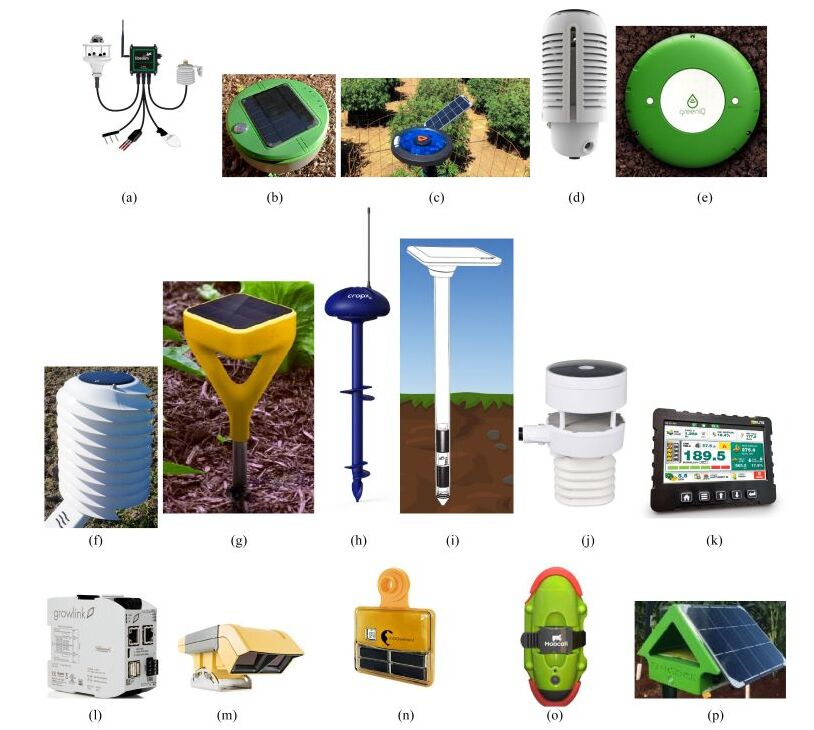
\includegraphics[width=6in]{screen.jpg}
    \caption{\textsf{The structure of our tic-tac-toe implementation.}}
    \label{fig:ds}
\end{figure*}
relies
on water and nutrients [20]. Aquaponic combines cultivating fish with hydroponics where the aquaculture water is
provided to hydroponically grown plants [21]. Recent agricultural advances correspond to the synthetic technological
developments in traditional agricultural systems around the
world [22].
Although modern agricultural techniques have boosted food
production and helped the world to cope with hunger crisis,
they have also drastically increased health calamities [23]. For
instance, the usage of modern pesticides reduces the antioxidant levels which may lead to neurodegeneration, cardiovascular, respiratory, renal, endocrine, cancer, and reproductive
problems [24]. Thus, researchers have started to re-examine
and review modern agricultural practices.
Recent advances and usage of information and communications technologies (ICTs) in the agricultural sector have
brought about numerous benefits and have paved the way
toward smart agriculture in both outdoor and indoor environments. ICTs can be used in the various agricultural sectors, such as cultivation, harvesting, irrigation, and farming.
ICTs help in improving the production efficiency, production
quality, post-harvesting processes, and monitoring of the environmental parameters that affect the agriculture ecosystem.
}
\end{multicols}

\vspace{10mm}


\end{document}
